\usetikzlibrary{chains}

\begin{frame}{x86 instruction encoding}
\begin{itemize}
    \item in 2110, 3330 you learned a ``teaching'' machine code
    \item Y86 (3330) is very like what x86 should be
    \item \ldots but it isn't
    \item why? history!
\end{itemize}
\end{frame}

\begin{frame}{the 8086}
\begin{tikzpicture}[overlay,remember picture]
\node[anchor=north east] {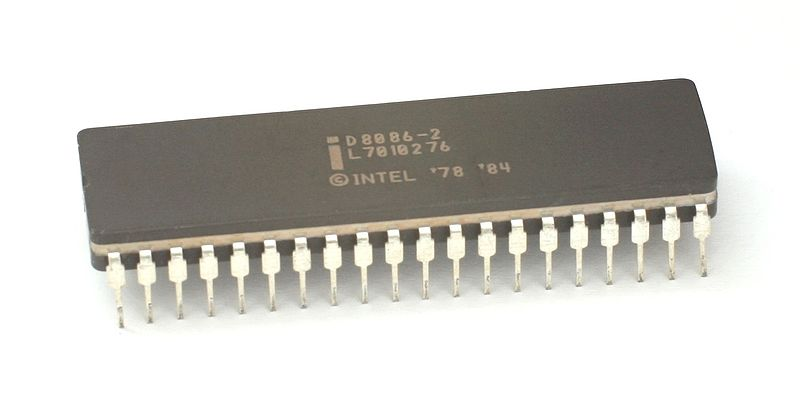
\includegraphics[width=0.3\textwidth]{../x8664-encoding/Intel8086}};
\end{tikzpicture}
\begin{itemize}
    \item 1979 Intel processor
    \item 4 general purpose 16-bit registers: AX, BX, CX, DX
    \item 4 special 16-bit registers: SI, DI, BP, SP
\end{itemize}
\end{frame}

\begin{frame}{8086 instruction encoding: simple}
\begin{itemize}
    \item special cases: 1-byte instructions:
    \begin{itemize}
    \item anything with no arguments
    \item push ax, push bx, push cx, \ldots (dedicated opcodes)
    \item pop ax, \ldots
    \end{itemize}
\end{itemize}
\end{frame}

\begin{frame}{8086 instruction encoding: two-arg}
\begin{itemize}
    \item 1-byte opcode
    \item sometimes {\tt ModRM} byte:
        \begin{itemize}
        \item 2-bit ``mod'' and 
        \item 3-bit register number (source or dest, depends on opcode) and
        \item 3-bit ``r/m'' (register or memory)
        \end{itemize}
    \item ``mod'' + ``r/m'' specify one of:
        \begin{itemize}
        \item {\tt \%reg} (mod = {\tt 11})
        \item {\tt (\%bx/\%bp, \%si/\%di)}
        \item {\tt (\%bx/\%si/\%di)}
        \item {\tt offset(\%bx/\%bp/,\%si/\%di)} (8- or 16-byte offset)
        \end{itemize}
    \item non-intuitive table
\end{itemize}
\end{frame}

\begin{frame}{16-bit ModRM table}
\begin{tikzpicture}
\node (table) {
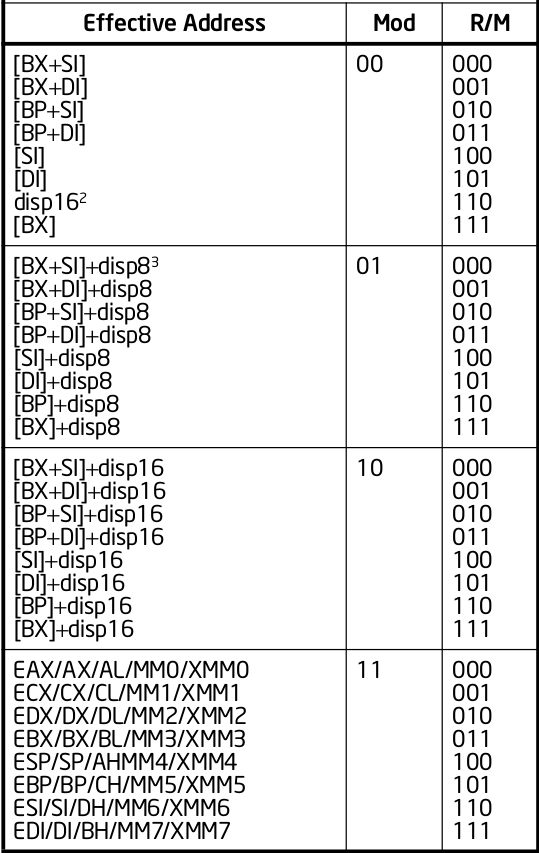
\includegraphics[height=0.8\textheight]{../x8664-encoding/16bitmodrm}
};
\begin{visibleenv}<2>
\node[anchor=north west,align=left] at (table.north east) {
    e.g. \texttt{add \%bl, \%cl} \\
    (Intel syntax: \texttt{add CL, BL}) \\
    Intel manual: \\
    \texttt{02 /r}: \texttt{ADD r8 {\normalfont(dest)}, r/m8} \\
    \texttt{/r} means ModRm byte with reg set to reg\# \\
    ~ \\
    opcode = \texttt{0x02}
    ModRM byte = \\
    \texttt{11} (mod) / \texttt{001} (reg: \%cl) / \texttt{011} (r/m: \%bl) \\
    or \texttt{1100 1011}
    ~ \\
    final encoding: \texttt{02 cb}
};
\end{visibleenv}
\end{tikzpicture}
\end{frame}

\begin{frame}{8086 evolution}
\begin{itemize}
\item Intel 8086 --- 1979, 16-bit registers
\item Intel (80)386 --- 1986, 32-bit registers
\item AMD K8 --- 2003, 64-bit registers
\end{itemize}
\end{frame}

\begin{frame}{x86 modes}
\begin{itemize}
\item x86 has multiple \myemph{modes}
\item maintains compatiblity
\item e.g.: modern x86 processor can work like 8086
    \begin{itemize}
    \item called ``real mode''
    \end{itemize}
\item different mode for 32-bit/64-bit
\item same basic encoding; some sizes change
\end{itemize}
\end{frame}

\begin{frame}{32-bit ModRM table}
\begin{tikzpicture}
\node (table) {
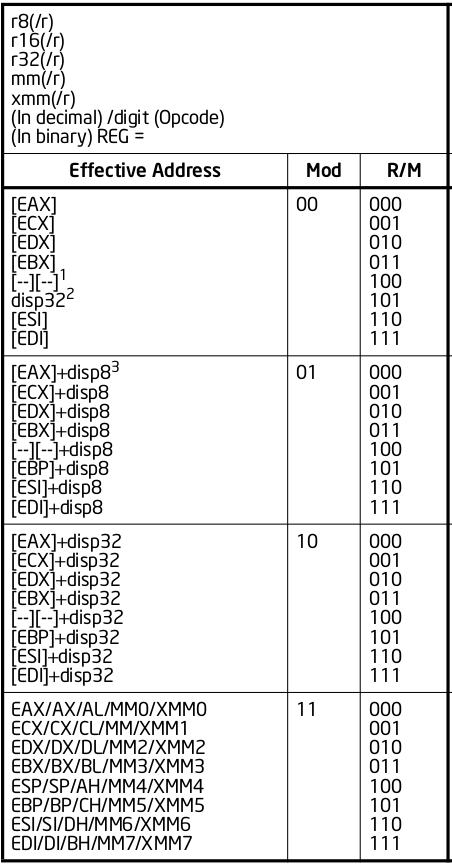
\includegraphics[height=0.8\textheight]{../x8664-encoding/32bitmodrm}
};
\begin{visibleenv}<2>
\node[anchor=north west,align=left] at (table.north east) {
    general pattern for 32-bit x86 register numbering: \\
    AX = 0, CX, DX, BX, SP, BP, SI, DI = 7 \\
    ~ \\
    not all registers treated equally to make space for \\
    special types of addressing: \\
    (base + index * scale, constant address)
};
\end{visibleenv}
\end{tikzpicture}
\end{frame}

\begin{frame}{32-bit addition: SIB bytes}
\begin{itemize}
\item 8086 addressing modes made registers different
\item 32-bit mode got rid of this (mostly)
\item problem: not enough spare bits in {\tt ModRM} byte
\item solution: if ``r/m'' bits = {\tt 100} (4, normally ESP), extra ``SIB'' byte:
    \begin{itemize}
    \item 2 bit \myemph<2>{scale}: {\tt 00} is 1, {\tt 01} is 2, {\tt 10} is 4, {\tt 11} is 8
    \item 3 bit \myemph<3>{index}: index register number
    \item 3 bit \myemph<4>{base}: base register number
    \end{itemize}
\item {\tt (\myemph<4>{\%baseReg},\myemph<3>{\%indexReg},\myemph<2>{scale})}
\end{itemize}
\end{frame}

\begin{frame}{intel manual: SIB table}
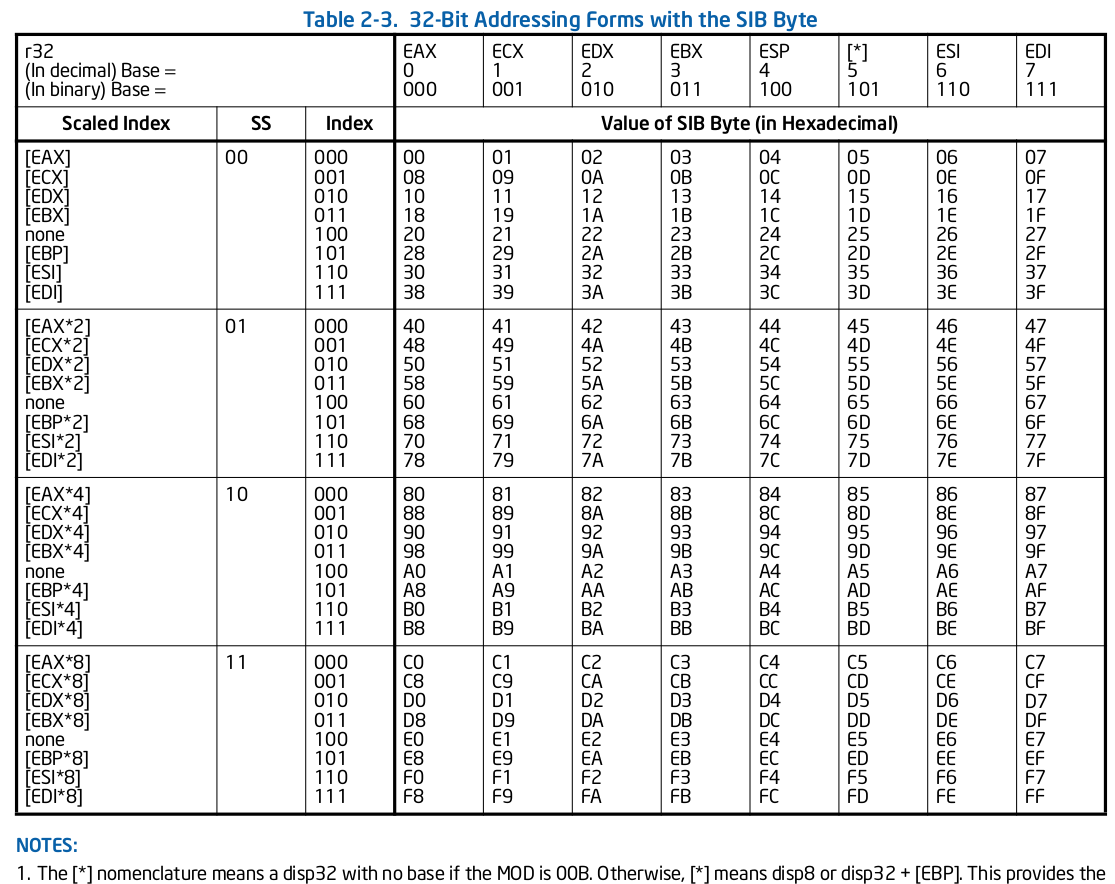
\includegraphics[height=0.9\textheight]{../x8664-encoding/32bitsib}
\end{frame}

\begin{frame}{basic 32-bit encoding}
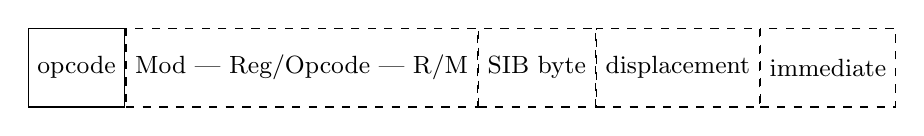
\begin{tikzpicture}
\begin{scope}[start chain=going right,node distance=0mm,every node/.style={on chain,draw,font=\small,minimum height=1cm}]
\node { opcode }; \node[dashed] { Mod | Reg{\fontsize{9}{10}\selectfont/Opcode} | R/M }; \node[dashed] {SIB byte}; \node[dashed] {displacement}; \node[dashed] {immediate};
\end{scope}
\end{tikzpicture}
\begin{itemize}
\item dashed: not always present
\item opcodes: 1-3 bytes
    \begin{itemize}
    \item some 5-bit opcodes, with 3-bit register field
    \item (alternate view: 8-bit opcode with fixed register)
    \item sometimes Reg part of ModRM used as add'tl part of opcode
    \end{itemize}
\item displacement, immediate: 1, 2, or 4 bytes
    \begin{itemize}
    \item or, rarely, 8 bytes
    \end{itemize}
\end{itemize}
\end{frame}

